%!TEX root = ../paper.tex

\section{Solution Architecture}
\label{sec:solution_architecture}
% Main components: Mobile apps, web app, BaaS, Beacons
After explained how is the experience of the Smart Restaurant for waiters,
customers and owners, the main components of the solution will be described,
the technologies that were used and how they interact with each other.
Figure~\ref{fig:architecture_base} shows the main components that were
implemented in order to be able to offer the Smart Restaurant experience,
described in section \ref{sec:smart_restaurant_experience}.
Also, for each component we point out the type of user that will interact
with it.
As the figure shows, the main components are the following:
\begin{description}
  \item[iBeacons]: The BLE beacons that use the iBeacon protocol explained
  in section \ref{sec:introduction}
  \item[Backend]: Which will store persistent data about the restaurants,
  such as, the restaurants' menus, the orders, and the mapping between
  the tables and the beacons' identifiers
  \item[Smartphone] Where will run the mobile apps, for the customers
  and for owners (described in section \ref{sec:smart_restaurant_experience})
  \item[Web application]: The waiters will use this to check the
  customers' orders.
\end{description}

\begin{figure}[!ht]
  \centering
    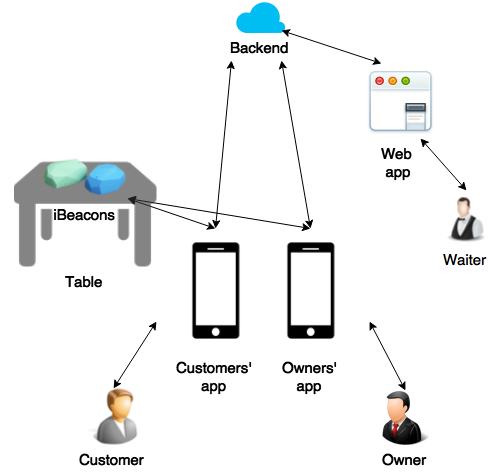
\includegraphics[width=0.7\textwidth]{figures/architecture_base}
    \caption{Main components of Smart Restaurant solution}
    \label{fig:architecture_base}
\end{figure}

\subsection{Backend}
\label{sub:backend}
The backend is the component that supports the mobile and web applications
that are used by the three main groups of users. It stores the data that is
needed for the other applications. This component was not implemented from
scratch, because we only need to be able to store persistent data and to
retrieve it. Instead of writing all the code to create the backend, we
are using a Backend as a Service (BaaS), which is Parse\footnote{http://parse.com}
\cite{parse}.
We only needed to create the collections and their structure.
It offers a REST API\cite{restful} that allow to perform the
Create Read Update and Delete (CRUD) operations
on the collections.
It also offers Software Development Kits (SDKs) for many platforms.
In our implementation we used the
Android\footnote{http://www.android.com} and
Javascript\footnote{http://developer.mozilla.org/en-US/docs/Web/JavaScript/About\_JavaScript}
SDKs. The Android SDK was used in the mobile apps (see \ref{sub:mobile_apps})
and the Javascript SDK was used in the web application
(see \ref{sub:web_app_for_waiters}).

\subsection{Mobile Apps}
\label{sub:mobile_apps}
% Two mobile apps
% (owners and customers)
% Technologies: App Android, BaaS Parse.com
% Package diagram
% Layer diagram for lib
As it is mentioned in section \ref{sec:smart_restaurant_experience}, our
solution for Smart Restaurants has two mobile apps. One for customers and
another one for Owners. Both are Android applications. Both apps are
part of the same project. The project is organized according to the
package diagram in figure~\ref{fig:package_diagram_android}, that shows
that the Android project is composed by three modules:
\begin{description}
  \item[lib]: Library that offers an API to scan for nearby beacons and
  to fetch data from and to the backend. This library uses the Parse Android
  SDK.
  \item[ownersapp]: Android app for restaurants' owners. This app uses
  the lib module to be able to scan for beacons and to get the relevant
  data from the backend
  \item[clientapp]: Android app for customers. This app also uses the lib
  module.
\end{description}

\begin{figure}[!ht]
  \centering
    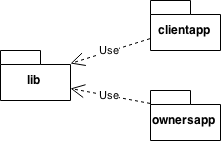
\includegraphics[width=0.4\textwidth]{figures/package_diagram_android}
    \caption{Package diagram of the Android project}
    \label{fig:package_diagram_android}
\end{figure}

The ownersapp and clientapp use the lib module to handle the beacons and
the communication with the backend. They only implement the user interface
and use the lib. Figure~\ref{fig:android-uml} shows the main classes
that implement the lib's logic that are the following:
\begin{description}
  \item[BeaconsManager]: Handles the beacons and offers methods to
  start scanning and stop the current scan process.
  \item[DataStore]: This class implements methods to fetch data from and to
  the backend, for instance, to login the user. These methods receive a callback
  that handles the result because the requests to the backend are asynchronous,
  which means that the user interface does not block waiting for the
  response.
  \item[DataStoreCallback]: This is used by most of the methods in DataStore
  class. This offers an interface that each specific backend's response
  handling should implement.
  \item[DataStoreObject]: Since we have speficied, in the backend, which
  collections we have and their structure, we have classes, that inherit from
  this one, that are wrappers for the raw data that comes from the backend.
\end{description}

\begin{figure}[!ht]
  \centering
    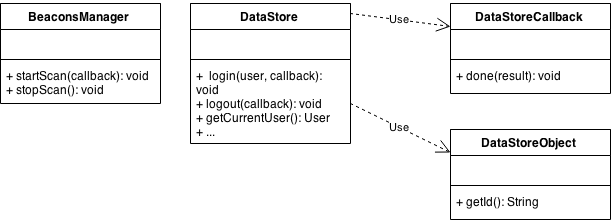
\includegraphics[width=0.8\textwidth]{figures/android-uml}
    \caption{Main classes of the lib module}
    \label{fig:android-uml}
\end{figure}

\subsection{Web App for Waiters}
\label{sub:web_app_for_waiters}
% Web app for waiters
% Technologies used: meteor, BaaS
% meteor: web sockets, live
As mentioned before, there is a web application for waiters. They can
check the coming orders.
This application was implemented using the
Meteor\footnote{http://www.meteor.com}\cite{meteor} framework which allows developers
to write web applications using Javascript in both client and server side.
Using this framework we can set up a new application issuing a single command.
It uses websockets\cite{websockets} to offer reactivity, which means,
when the data changes on the server,
the client will be automatically updated, so the users do not need to
refresh the web page in order to see the updates. We chose to use this
because it allows rapid prototyping and the reactivity feature is important
because, this waiters, only need to look at the screen to know which
orders they have to process next.
